\documentclass{article}

\usepackage[T1]{fontenc} 
\usepackage[utf8]{inputenc}
\usepackage[polish]{babel}

\usepackage{hyperref}


\renewcommand{\contentsname} {Spis treści}

\usepackage{graphicx}

\begin{document}
 
\begin{titlepage} 
	\newcommand{\HRule}{\rule{\linewidth}{0.5mm}} 
	
	\center 
	
	\textsc{\LARGE POLITECHNIKA WROCŁAWSKA} \\[0.5cm]
	\textsc{\LARGE WYDZIAŁ ELEKTRONIKI} 
	
	\HRule\\[3.0cm]
	
	{\huge Projekt z rozproszonych i obiektowych systemów baz danych}\\[2.0cm] 
	
	{\huge\bfseries Rozproszony system bazodanowy przeznaczony do obsługi oddziałów restauracji}\\[2.0cm] 
	
	
	

	\begin{minipage}{0.4\textwidth}
		\begin{flushleft}
			\large
			\textit{AUTORZY}\\
			Michał Kalinowski\\
			Paweł Kolak\\
			Dawid Mikowski\\
		\end{flushleft}
	\end{minipage}
	~
	\begin{minipage}{0.4\textwidth}
		\begin{flushright}
			\large
			\textit{PROWADZĄCY}\\
			Dr inż. Robert Wójcik
			W4/K9
			\\[2.0cm] 
			OCENA PRACY:
		\end{flushright}
	\end{minipage}
	
	% If you don't want a supervisor, uncomment the two lines below and comment the code above
	%{\large\textit{Author}}\\
	%John \textsc{Smith} % Your name
	
	%------------------------------------------------
	%	Date
	%------------------------------------------------
	
	\vfill\vfill\vfill % Position the date 3/4 down the remaining page
	\HRule\\[0.5cm]
	{\large\today} % Date, change the \today to a set date if you want to be precise
	
	%------------------------------------------------
	%	Logo
	%------------------------------------------------
	
	%\vfill\vfill
	%\includegraphics[width=0.2\textwidth]{placeholder.jpg}\\[1cm] % Include a department/university logo - this will require the graphicx package
	 
	%----------------------------------------------------------------------------------------
	
	\vfill % Push the date up 1/4 of the remaining page
	
\end{titlepage}
\clearpage

\tableofcontents
\newpage
\listoffigures

 \newpage
\section{Wstęp}
	\subsection{Cele projektu jest}
	Projekt ma na celu zaprojektowanie oraz implementację aplikacji umożliwiającej dostęp do rozproszonej bazy danych sieci restauracji, oraz konfigurację tejże bazy danych. Projekt zakłada wykorzystanie rozproszonej bazy danych celem zwiększenia wydajności systemu. Baza danych stworzona w ramach projektu ma być zlokalizowana na trzech serwerach bazodanowych. Dane będą replikowane od serwera głównego do serwerów klienckich. Użytkownicy będą mieli dostęp do bazy danych restauracji za pośrednictwem dwóch typów aplikacji: klienckiej i administracyjnej.
	
	\subsection{Zakres projektu}
	\paragraph{}
	Zadania projektowe podzielone zostały na trzy rozłączne obszary tematyczne. Pierwszy z nich dotyczył czynności związanych z bazą danych. Została stworzona i skonfigurowana rozproszona baza danych przy pomocy SQL Server firmy Microsoft. Baza znalazł się w trzech odrębnych instancjach sql serwera. Zaprojektowany został fizyczny model bazy oraz dane początkowe. Zrealizowana została replikacja transakcyjna typu master - salve do dwóch serwerów klienckich. Wykonane zostały również testy funkcjonalne replikacji oraz testy wydajnościowe. Baza danych przechowuje tabele opisujące takie dane jak restauracje, lokacje, menu, dania i promocje. Każdy z trzech serwerów zawsze zawiera ten sam zestaw danych co pozostałe serwery. Zmiana dokonana na głównym serwerze widoczne są równocześnie na wszystkich serwerach.
	\paragraph{}
	Kolejnym obszarem była warstwa logiki biznesowej która dotyczy wykonywania operacji na bazie danych. Projekt zakłada zaimplementowanie aplikacji serwerowej opartej o .Net Core oraz web API.  W ramach projektu skonfigurowano serwer IIS oraz połączenie aplikacji z bazą danych. 
	\paragraph{}
	Ostatni zbiór zadań projektowych dotyczył umożliwienia użytkownikowi interakcji z systemem. Projekt zakładał stworzenie interfejsu użytkownika. Obszar ten w naszym przypadku został podzielony na dwie aplikacje. Jedna której zadaniem będzie obsługa klienta w restauracji, głównym zadaniem tej aplikacji będzie wyświetlanie menu. Drugą aplikacją będzie aplikacja administratorska która umożliwi modyfikację danych w bazie. Aplikacje dynamicznie pobiera dane z serwera oraz wykonuje operacje na bazie danych za pośrednictwem interfejsu udostępnionego przez aplikację serwerową. Tą część zrealizowaliśmy przy pomocy technologii Angular. 
	

	\subsection{Architektura systemu}  
	\paragraph{}
	W projekcie jest zrealizowany 3-warstwowy model komunikacji klient/serwer. W modelu tym przetwarzanie danych (funkcje biznesowe) są realizowane po stronie serwera internetowego, zarządzanie danymi - po stronie serwerów baz danych, natomiast po stronie klienta jest realizowana jedynie prezentacja danych z wykorzystaniem przeglądarki internetowej. Dostęp do aplikacji realizującej funkcje biznesowe będzie realizowany poprzez podanie adresu serwera WWW.
	\paragraph{}
	W projekcie wykorzystywane są jednorodne bazy danych (tj. wszystkie bazy danych będą tego samego typu). Dostęp do baz danych realizowany będzie w oparciu o funkcje aplikacji, które komunikują się bezpośrednio z odpowiednimi serwerami bazodanowymi. W warstwie rozproszonej bazy danych zrealizowany zostanie mechanizm umożliwiający replikację informacji pomiędzy węzłami.
	\paragraph{}
	W ramach projektu wykorzystana została replikacja transakcyjna. W tym podejściu istnieje kilka instancji aplikacji oraz serwera bazodanowego, na serwerze master możliwy jest odczyt i zapis, natomiast na pozostałych dwóch serwerach typu slave możliwy jest jedynie odczyt. Prawa do poszczególnych baz dla instancji aplikacji serwerowej zostały tak przydzielone, aby niemożliwy był zapis na serwerach slave, Prawo do zapisu udostępnione jest jedynie użytkownikowi mającemu dostęp do aplikacji administracyjnej, która podłączona jest do głównego serwera bazodanowego.

 
\section{Replikacja w systemie bazy danych}
	\subsection{Pojęcie replikacji i podstawowe informacje}
	\paragraph{}
\textbf{Replikacja danych} – proces powielania informacji pomiędzy różnymi serwerami baz danych. Można rozróżnić następujące rodzaje replikacji:
	\begin{itemize}
	
\item	Replikacja migawkowa (ang. snapshot replication) – rozprowadzane dane mają stan z pewnego określonego momentu w czasie. Ten rodzaj replikacji znajduje głównie zastosowanie przy danych, które nie są często modyfikowane, jednak modyfikacje te mogą być znaczne. Zmiany pomiędzy kolejnymi wykonywanymi migawkami nie są monitorowane.
\item	Replikacja transakcyjna lub przyrostowa (ang. transaction replication) – dane rozprowadzane są na podstawie logów transakcji, dane modyfikowane są tylko na głównym serwerze.
\item	Replikacja dwukierunkowa lub łącząca (ang. merge replication) – dwukierunkowe rozprowadzanie danych; serwer realizuje transakcje zarówno od innego serwera, jak i od klientów. Transakcje realizowane przez klientów mogą być również przeprowadzone bez połączenia pomiędzy serwerami, jednak w takim przypadku w czasie synchronizacji może dojść do konfliktu, który musi być rozwiązany przez osobę przeprowadzającą aktualizację.

	\end{itemize}

Replikacja w SQL Serwerze oparta jest na technice publikacji i subskrypcji danych. Serwer udostępniający dane jest publikatorem danych. Przesyła on kopie wszystkich zmian opublikowanych danych do serwera zajmującego się dystrybucja, tzw. dystrybutora.
Dystrybutor zawiera bazę dystrybucji, która otrzymuje wszelkie zmiany wprowadzane w danych, przechowuje je i przesyła do serwerów subskrypcji (subskrybentów), obsługujących bazę docelową, która odbiera opublikowane dane i przechowuje ich kopię.
Subskrybent może pobierać wszystkie dane publikowane przez serwer źródłowy lub tylko ich część. Serwer dystrybucji i publikator mogą być na tym samym komputerze lub na innych.

\paragraph{}
Komponenty replikacji są następujące:
	\begin{itemize}
\item	\textbf{Publikator} – serwer udostępniający dane innym serwerom. Przechowuje dane o wszystkich publikacjach dokonanych w bazie danych.
\item	\textbf{Dystrybutor} – serwer zawierający bazę zarządzającą dystrybucją danych
\item	\textbf{Subskrybent} - serwer przechowujący kopie publikacji i przesyłający lub odbierający zmiany od publikatora. Może być również publikatorem dla innych subskrybentów.
\item	\textbf{Artykuł} – zbiór danych, który ma być replikowany i może zawierać dane przechowywanej procedury lub tablicy przeznaczonej do replikacji.
\item	\textbf{Publikacja} – zbiór jednego lub wielu artykułów. Subskrybenty subskrybują publikacje, a nie artykuły.
10
\item \textbf{Subskrybcja} – tworzona jest w celu pobrania publikacji przeznaczonych do replikacji

\end{itemize}

\paragraph{}
Replikacja transakcyjna opiera się w głównej mierze na tzw. agentach. Są to exe'ki, które mogą być uruchamiane z wiersza poleceń, aczkolwiek w większości scenariuszy uruchamia je SQL Server Agent za pomocą Jobów. Poniżej znajduje się lista agentów biorących udział w opisywanym rodzaju replikacji transakcyjnej. Lista ta nie uwzględnia wszystkich agentów związanych z replikacją w MS SQL Server.
\begin{itemize}
\paragraph{}
\item 
Log Reader Agent - agent (logread.exe) który jest odpowiedzialny za cykliczne odczytywanie logu transakcyjnego publikacyjnej bazy danych w poszukiwaniu transakcji przeznaczonych do replikacji i przekazywaniu ich do Dystrybutora.
Snapshot Agent - agent (snapshot.exe) odpowiedzialny za generowanie snapshotów obiektów bazy publikacyjnej ( jest np. wykorzystywany przy inicjalizowaniu subskrypcji ze snapshotów).
\paragraph{}
\item
Agent Dystrybucji (Distribution Agent) - agent (distrib.exe) odpowiedzialny za aplikowanie replikowanych transakcji oraz snapshotów do tabel subskrybenta. Zródłem danych dla agenta jest baza dystrybucyjna. Agent może być uruchamiany na subskrybencie (Pull Subscription) albo na dystrybutorze (Push Subscription).
\end{itemize}

	\begin{figure}[hbt!]
		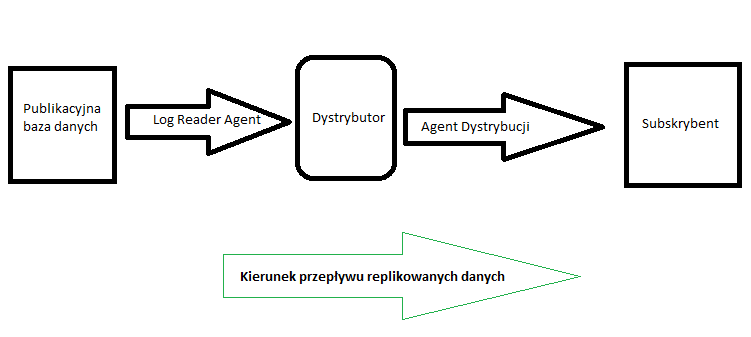
\includegraphics[width=8cm]{Files/Pictures/ReplikacjaArchitektura}
		\centering
		\caption{Schemat replikacji}
	\end{figure}

	\subsection{Replikacja transakcyjna}
	\paragraph{} Replikacja transakcyjna jest replikacją synchroniczną, szczególnie efektywną, gdy chcemy zmniejszyć ilość replikowanych danych, ponieważ zmiany są replikowane na podstawie logu transakcyjnego. W przypadku replikacji transakcyjnej wszelkie modyfikacje bazie w postaci danych w tabeli jak i zmian na strukturze tabel są propagowane do subskrybentów. Podczas transakcji na serwerze master. Wszystkie zmiany trafiają do dziennika transakcji i tam oczekują na wysłanie ich do subskrybentów jeśli są dla nich przeznaczone. Przesyłane są tylko transakcje zrealizowane, a użytkownicy nie są wyłączeni z korzystania z tablic, w czasie ich aktualizacji. Technika ta pozwala zachować spójność transakcyjną. Dziennik transakcji bazy danych publikatora przechowuje transakcje przeznaczone do replikacji, dopóki nie zostaną przeniesione do bazy dystrybutora, a następnie zostaje oczyszczony tak, że zostają w nim tylko transakcje, które nie są przeznaczone do replikacji.
	
\newpage
\section{Model konceptualny i fizyczny bazy danych}
	\subsection{Model konceptualny}

\begin{figure}[hbt!]
				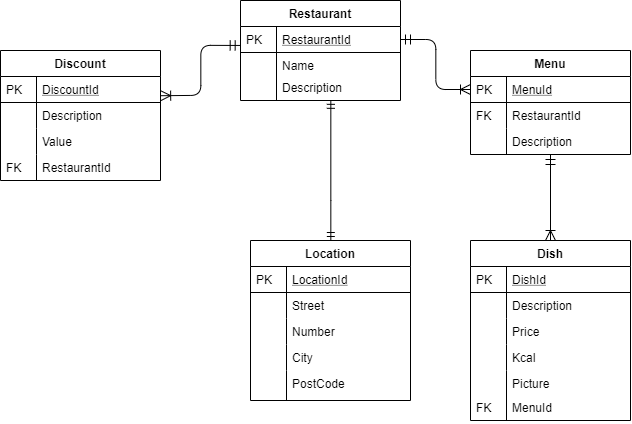
\includegraphics[width=10cm]{Files/Pictures/Model_K}
				\centering
				\caption{Model konceptualny}
			\end{figure}
	\subsection{Model fizyczny}

\begin{figure}[hbt!]
				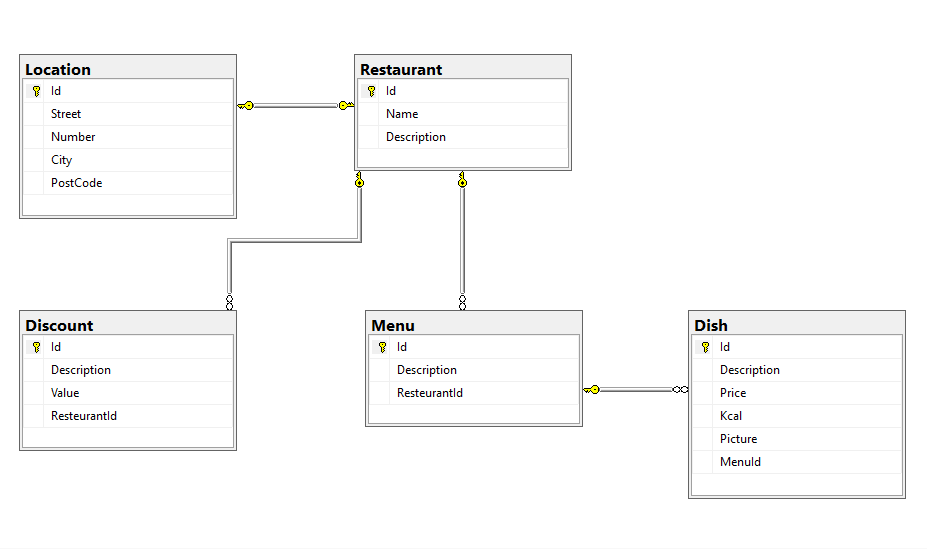
\includegraphics[width=10cm]{Files/Pictures/Model}
				\centering
				\caption{Model fizyczny}
			\end{figure}
	
	\subsection{Model replikacji}	
	System ma służyć klientom sieci restauracji do przeglądania menu w poszczególnych restauracjach. Jeden węzeł główny ma możliwość modyfikacji, do niego dostęp jest poprzez aplikację administratorską która umożliwia modyfikacje wartości w bazie. Na kolejnych dwóch węzłach użytkownicy mają jedynie prawo odczytu, na tych połączone są aplikacje klienckie. Na węźle nadrzędnym uruchomiony jest publisher który nadzoruje rozgłaszanie logów transakcyjnych. Również na głównej bazie znajdują się subskrybenci którzy odpowiadają za przyjmowanie danych na bazach docelowych. Zostały one umieszczone po stronie bazy głównej, MS Serwer umożliwia umieszczenie ich również po stronie subskrybentów.
	
	
	
	\begin{figure}[hbt!]
		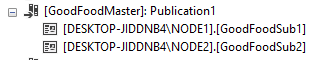
\includegraphics[width=8cm]{Files/Pictures/repSub}
		\centering
		\caption{Konfiguracji replikacji}
	\end{figure}
	

\newpage
\section{Implementacja bazy danych w środowisku}
	\subsection{Realizacja bazy danych}
	
	\subsection{Wykorzystanie mechanizmów replikacji transakcyjnej}
System został stworzony na jednej maszynie, na której umieszczone zostały 3 instancji Microsoft SQL Server 2017. Taka możliwość nie wymaga podziału na kontenery, jest to wspierana przez Microsoft możliwość. Konieczny jest jedynie wybór odpowiedniej ścieżki instalacji.
	
	\begin{figure}[hbt!]
		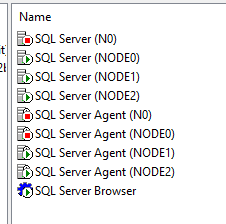
\includegraphics[width=8cm]{Files/Pictures/instancje}
		\centering
		\caption{Instancje serwera}
	\end{figure}
	

	
	Następnym krokiem który należy przygotować przed uruchomieniem replikacji jest przejście instrukcji przygotowanego przez producenta. Czynności które zaleca wykonać producent to:
	
	\begin{itemize}
	\item	\textbf{Przygotowanie odpowiednich kont} – Microsoft zaleca stworzenie kont z odpowiednimi zabezpieczeniami
	\item	\textbf{Utworzenie folderu} – Konieczne jest stworzenie folderu w którym znajdować się będą 	pliki tym czasowe bazy oraz obrazy. Folder musi mieć odpowiednio ustawione opcje udostępniania w sieci oraz prawa użytkowników dla każdego z użytkowników.
	\end{itemize}
	
	Replikacja transakcyjna została skonfigurowana przy pomocy narzędzia Microsoft SQL Server Management Studio. Na początku na serwerze master została utworzona i wypełniona początkowymi danymi. Następnie na pierwszej instancji – Node0 został uruchomiony dystrybutor oraz publikacja zawierająca całą bazę danych aplikacji restauracji.
	
	\begin{figure}[hbt!]
		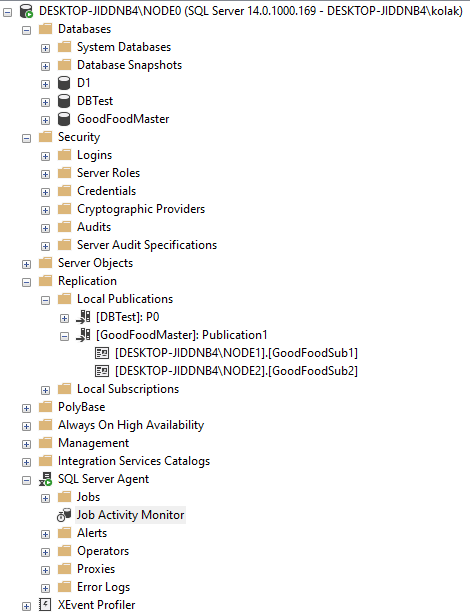
\includegraphics[width=8cm]{Files/Pictures/postawionaReplikacja}
		\centering
		\caption{Urochomiony publisher i subscriber}
	\end{figure}
	
	MS SQL Serwer w przypadku replikacji transakcyjnej udostępnia możliwość uruchomienia subskrybentów zarówno po stronie mastera jak i klienta. W naszym przypadku wybraliśmy pierwszą opcje. Podczas implementacji subskrypcje utworzyły po swojej stronie instancje baz do których będą replikowane dane. Istotnym elementem jest dodanie prawa do nowopowstałych baz na instancjach SQL Serwera użytkownikom których konta zostały użyte w konfiguracji subskrypcji. Po utworzeniu 
	
	
	\newpage	

\section{Projekt i implementacja aplikacji}
Na poniższym schemacie została pokazana struktura systemu. W celu zrealizowania założeń zaimplementowane zostały dwie aplikacje dostępowe dla dwóch różnych typów odbiorców (klient, administraotr).

			\begin{figure}[hbt!]
				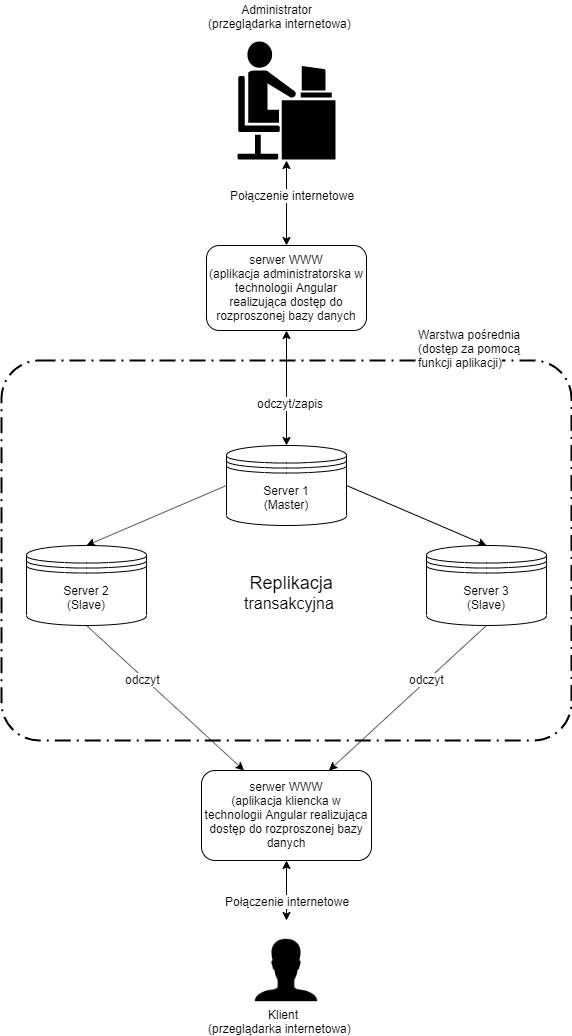
\includegraphics[width=8cm]{Files/Pictures/SystemStruct}
				\centering
				\caption{Diagram przypadków użycia}
			\end{figure}
			\newpage
	\subsection{Aplikacja (Backend)}
	Backend służy jako wygodny w użyciu interfejs dostępu do bazy danych zwracając potrzebne informacje w formacie JSON.
		\subsubsection{Technologie}
		Aplikacja backendowa została napisana w języku C\# jako .Net Core Api w wersji 2.2. Dostęp do bazy danych zaimplementowany został wykorzystując ORM Entity Framework, który pozwala w prosty wykonywać operacje na tabelach tj. dodawanie elementów, usuwanie elementów.
		\subsubsection{Model}
			Model wykorzystywany w api odpowiada strukturze bazy danych zapisanej w języku C\#
			\begin{figure}[hbt!]
				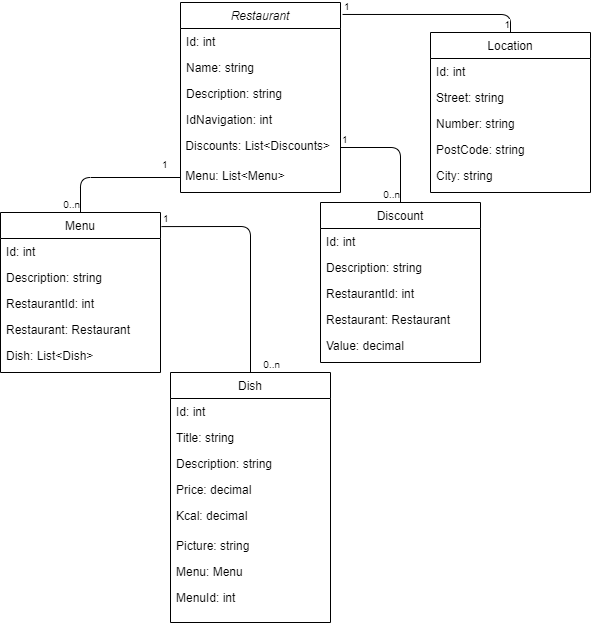
\includegraphics[width=8cm]{Files/Pictures/DiagramKlas}
				\centering
				\caption{Diagram klas aplikacji backendowej}
			\end{figure}
		\subsubsection{Kontrolery}
		Aplikacja pozwala użytkownikowi na korzystanie z 4 różnych kontrolerów:
			\begin{itemize}
				\item \textbf{Discount Controller} 
					\begin{itemize}
						\item \textbf{GET} \textit{api/Discount/id}	- zwraca informacje o promocji z podanym id	
						\item \textbf{POST} \textit{api/Discount} - dodaje promocję do bazy danych
						\item \textbf{DELETE} \textit{api/Discount/id}	 - usuwa promocję o podanym id				
					\end{itemize}

				\item \textbf{Dish Controller}
					\begin{itemize}
						\item \textbf{GET} \textit{api/Dish/id} - zwraca informacje o daniu z podanym id
						\item \textbf{POST} \textit{api/Dish} - dodaje danie do bazy danych
						\item \textbf{DELETE} \textit{api/Dish/id} - usuwa danie o podanym id
					\end{itemize}
					
				\item \textbf{Menu Controller}
					\begin{itemize} 
						\item \textbf{GET} \textit{api/Menu/id} - zwraca informacje o menu oraz pełną listą dań które się w nim znajdują
						\item \textbf{POST} \textit{api/Menu} - dodaje menu do bazy danych
						\item \textbf{DELETE} \textit{api/Menu/id} - usuwa menu o podanym id
					\end{itemize}
					
				\item \textbf{Restaurant Controller}
					\begin{itemize}
						\item \textbf{GET} \textit{api/Restaurant/id} - zwraca podstawowe informacje o restauracji z podanym id 
						\item \textbf{GET} \textit{api/Restaurant/Full/id} - zwraca wszystkie informacje o podanej restauracji (lokalizacja, promocje, menu)
						\item \textbf{GET} \textit{api/Restaurant/Discounts/id} - zwraca wszystkie promocje z restauracji o podanym id
						\item \textbf{GET} \textit{api/Restaurant/Dishes/id} - zwraca wszystkie dania z restauracji o podanym id
						\item \textbf{POST} \textit{api/Restaurant/} - dodaje restauracje do bazy danych
						\item \textbf{DELETE} \textit{api/Restaurant/id} - usuwa restauracje o podanym id 
					\end{itemize}
			\end{itemize}
		\subsubsection{Zachowanie wysokiej dostępności w przypadku awarii}
		W aplikacji rozwiązany jest także problem związany z możliwością awarii jednej z baz danych. Dzięki wykorzystaniu metody onConfiguring, która jest uruchamiana za każdym razem kiedy request zostaje odebrany przez aplikację jesteśmy w stanie wykonać próbę zapisu do jednej z baz i jeżeli się ona nie powiedzie zostaje wykorzystana inna.
	\newpage
\newpage
	\subsection{Aplikacja (Frontend - Admin)}
		\subsubsection{Funkcje aplikacji - diagram przypadków użycia}
		Na poniższym rysunku przedstawiono diagram przypadków użycia stworzonej aplikacji administratorskiej. Wszystkie przedstawione na diagramie funkcjonalności zostały zaimplementowane. Ze wsględu na cel projektu głównym celem było przedstawienie możliwości replikacji.
		Na poniższym rysunku przedstawiono diagram przypadków użycia stworzonej aplikacji administratorskiej. Wszystkie przedstawione na diagramie funkcjonalności zostały zaimplementowane. Ze wsględu na zakres projektu głównym celem było przedstawienie możliwości replikacji.
			\begin{figure}[hbt!]
				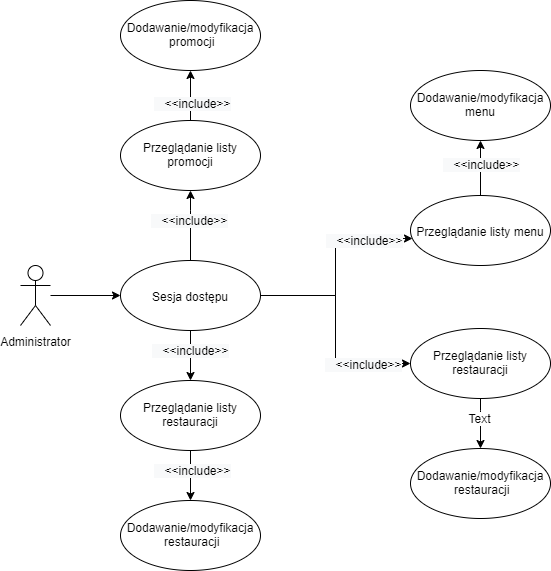
\includegraphics[width=8cm]{Files/Pictures/UMLAdminApp}
				\centering
				\caption{Diagram przypadków użycia}
			\end{figure}
		\subsubsection{Realizacja wybranych funkcjonalności}
		Aplikacja kliencka została zrealizowana w technologi internetowej z wykorzystaniem framework'u Angular 8.
		Aplikacja kliencka została zrealizowana w technologi internetowej z wykorzystaniem framework'u Angular 8, w którym użyte zostały technologie:  TypeScript, CSS, HTML, Bootstrap. Administrator może połączyć się z aplikacją za pomocą przeglądarki internetowej. Pierwszym widokiem jest ekran z listą dostępnych w sieci restauracji, z których można wybrać jedną z wymienionych. Dodatkowo zawarte są podstawowe informacje o wartościach, jakie firma respektuje. Następny widok jest związany z wyświetleniem szczegółowych wiadomości o wybranym lokalu (menu, promocje, adres). Akcje, jakie można wykonać z poziomu tego okna to:
		\begin{itemize}
				\item
					\textbf{prziejście do okna umożliwiającego odanie promocję,} 
				\item
					\textbf{prziejście do okna umożliwiającego odanie menu,}
				\item
					\textbf{przejscie do informacji o wybranym menu,}
				\item
					\textbf{usunięcie restauracji,}
				\item
					\textbf{usunięcie wybranej promocji.}
			\end{itemize}
			Analogicznie w widokach związanych z menu i daniem można dokonywać operacji  dodania oraz usunięcia wybranych elementów.

			\begin{figure}[hbt!]
				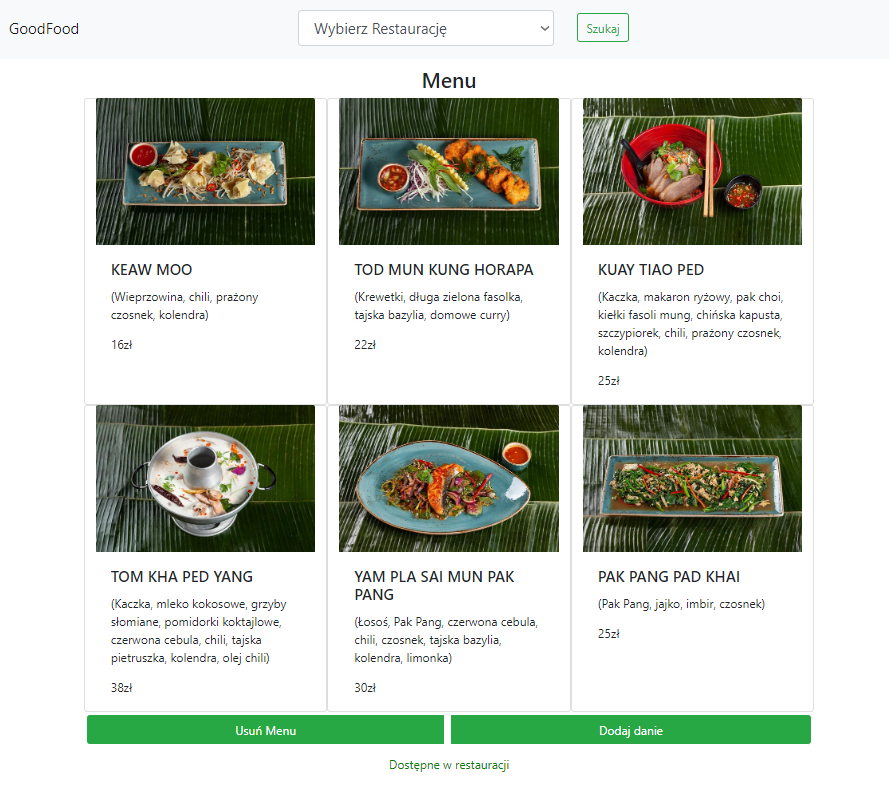
\includegraphics[width=8cm]{Files/Pictures/MenuList_A}
				\centering
				\caption{Widok informacji o menu}
			\end{figure}

			\begin{figure}[hbt!]
				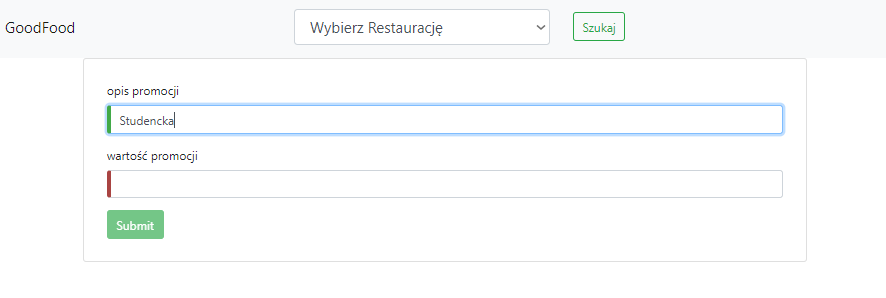
\includegraphics[width=8cm]{Files/Pictures/Add_A}
				\centering
				\caption{Widok dodawania obiektu przez administratora}
			\end{figure}

	\newpage
	\subsection{Aplikacja (Frontend - Customer)}

		\subsubsection{Funkcje aplikacji - diagram przypadków użycia}
		Na poniższym rysunku przedstawiono diagram przypadków użycia stworzonej aplikacji klienckiej. Podobnie jak w poprzedniej aplikacji zostały zaimplementowane wszystkie funkcjonalności.
			\begin{figure}[hbt!]
				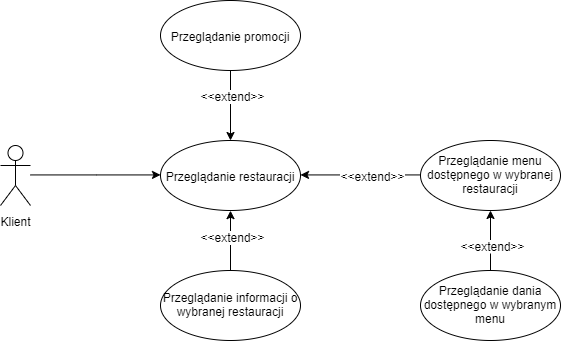
\includegraphics[width=10cm]{Files/Pictures/UMLCustomerApp}
				\centering
				\caption{Diagram przypadków użycia}
			\end{figure}
		\subsubsection{Realizacja wybranych funkcjonalności}	
		Aplikacja kliencka została zrealizowana w technologi internetowej z wykorzystaniem framework'u Angular 8.
		Aplikacja kliencka została zrealizowana w technologi internetowej z wykorzystaniem framework'u Angular 8, w którym użyte zostały technologie:  TypeScript, CSS, HTML, Bootstrap.
		Jest to aplikacja, która dokonuje jedynie odczytu. Została stworzona w celu informacyjnym dla klienta, który może znaleźć najważniejsze informacje o lokalach należących do sieci restauracji.
			\begin{figure}[hbt!]
				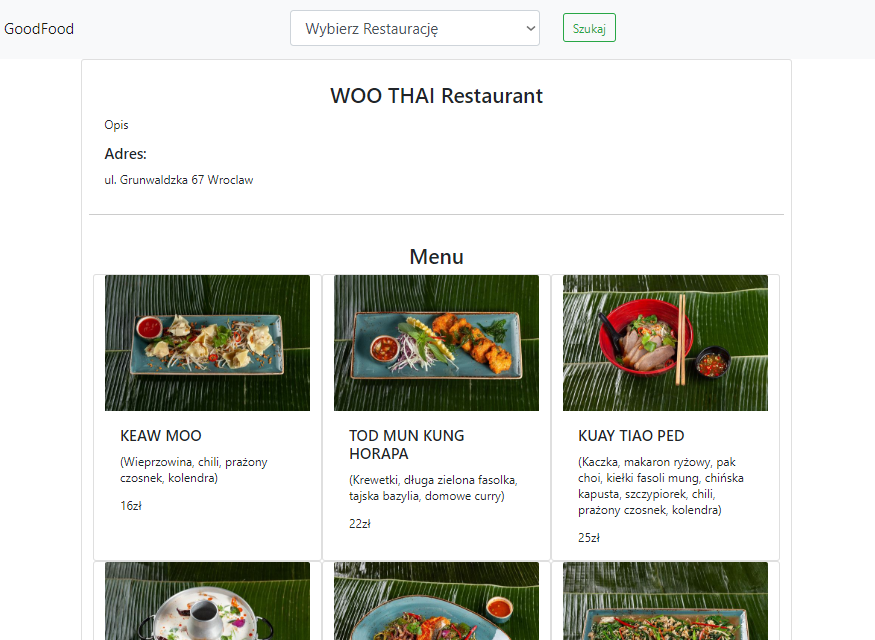
\includegraphics[width=8cm]{Files/Pictures/Info_C}
				\centering
				\caption{Widok informacji o restauracji}
			\end{figure}
\newpage
\section{Wdrożenie i testowanie aplikacji}
Prezentacja działania srodowiska wymagała specjalnego przygotowania i konfiguracji sieci lokalnej.
\subsection{Konfiguracja środowiska produkcyjnego}
	Wszystkie komputery znalazły się w sieci lokalnej. Na PC2 zostały skonfigurowane bazy danych w podstacji trzech instancji MS serwer, wraz z replikacjią między nimi. PC1 posiadał instancję aplikacji administratorskiej wraz z odpowiadającą jej aplikacją serwerową. PC3 posiadał natomiast aplikację kliencką.


	\begin{figure}[hbt!]
		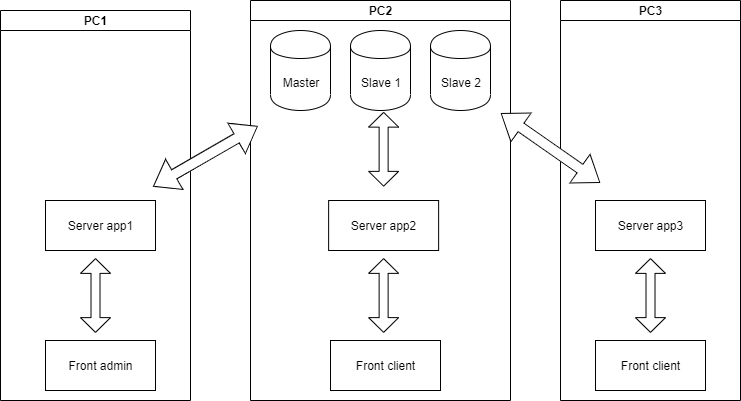
\includegraphics[width=8cm]{Files/Pictures/setup}
		\centering
		\caption{Środowisko testowe}
	\end{figure}

\subsection{Testowanie wybranych operacji}	
Dzięki konfiguracji możliwe było pokazanie w łatwy sposób modyfikację na PC1, odczyt zmodyfikowanych danych na PC3, z możliwością podglądu na żywo na PC2 danych transakcyjnych.	

\subsubsection{Test operacji dodawania i odczytu}	

Pierwszym etapem testów były pojedyncze operacje zapisu. Do bazy przez aplikację administracyjną były dodawane pojedyncze wpisy do poszczególnych tabel. Na subskrybentach było weryfikowane opóźnienie. Średni czas propagacji informacji pomiędzy węzłami wyniósł 1870ms.
Drugim etapem były testy dotyczące większej liczby wpisów, w naszym przypadku było to 10000. W tym przypadku opóźnienie wyniosło ok. 2000ms jednak widoczne były paczki transakcji które docierały na serwery slave po około 30 wpisów co 2-3ms. Jest to zjawisko związane prawdopodobnie z kwantowaniem informacji w transakcjach przez którąś ze stron.

\subsubsection{Testowanie działania w warunkach awarii}
Kolejnym etapem testów było pozbawianie systemu jednego z węzłów. Wyłączany był jeden z węzłów subskrybentów. Wykonywane były operacje dodawania na serwerze oraz obserwowane na aplikacjach klienckich. System zachował się zgodnie z założeniami, aplikacje serwerowe wykrywały uszkodzony węzeł i przekierowywały ruch do działającego. Po uruchomieniu wykluczonego serwera połączenie było wznawiane po ok. 7 sekundach od uruchomienia SQL server agenta.

\subsubsection{Wnioski z testów}
Testy potwierdziły niezawodność bazy i realizację założonych modeli zachowań. Działanie bazy jest adekwatne do architektury dla jakiej została stworzona. Potwierdzony został również niezawodność bazy w przypadku awarii jednego z węzłów. 

\newpage
\section{Podsumowanie}
W trakcie prac nad realizacją projektu udało się wykorzystać mechanizm replikacji
transakcyjnej i replikacji master-slave. Obsługa tych narzędzi do tworzenia bazy danych
okazała się łatwa i intuicyjna. Najwięcej problemów napotkano przy konfiguracji
praw dostępu do bazy oraz sama konfiguracja tego. Wybór stworzenia własnego środowiska wdrożeniowego oraz testowego zaoszczędziło grupie czas na inne zadania zawarte w projekcie.
Zrealizowana została również aplikacja kliencka i administratorska w technologii Angular łącząca się z bazą przez aplikację pośrednią zarządzającą dostępem do wybranych węzłów. Cały projekt zakończył się sukcesem, a działanie programu klienckiego spełnia wszystkie
wcześniejsze założenia.
\newpage
\section{Literatura}

\begin{thebibliography}{99}
\bibitem{pa} A. Jorgensen, B. Ball, S. Wort,:
\emph{Microsoft SQL Server 2014. Podręcznik administratora},
Helion
\bibitem{pa}
\emph{Dokumentacja MS SQL Servera}
\bibitem{pa} R. Wójcik
\emph{Wykłady},
2019
\bibitem{pa}
\href{https://angular.io/guide/forms}{Dokumentacja Angular 8 [Link]}
\bibitem{pa}
\href{https://getbootstrap.com}{Dokumentacja Bootstrap 4 [Link]}
\end{thebibliography}

 
\end{document}